\documentclass[12pt]{article}

\usepackage{tikz}
\usetikzlibrary{backgrounds}
\usepackage{xcolor}
\usepackage{listings}
\usepackage{caption}
\definecolor{lightgrey}{gray}{0.8}
\lstset{
    frame=LRBT
  , frameround=tttt
  , framerule = 0pt
  , classoffset = 0
  , backgroundcolor=\color{lightgrey}
  , frame=simple
  , rulesepcolor=\color{gray}
  , basicstyle=\color{black} }

\usepackage{graphicx}
\usepackage{amsmath}
\usepackage{amsthm}
\usepackage{amssymb}
\usepackage{url}
\usepackage{multirow}
\usepackage{times}
\usepackage{fullpage}
\usepackage{wrapfig}
\newcommand{\comment}[1]{}
\usepackage{fancyhdr}


\usetikzlibrary{backgrounds}
\makeatletter

\tikzset{%
  fancy quotes/.style={
    text width=\fq@width pt,
    align=justify,
    inner sep=1em,
    anchor=north west,
    minimum width=\textwidth,
  },
  fancy quotes width/.initial={.8\textwidth},
  fancy quotes marks/.style={
    scale=8,
    text=white,
    inner sep=0pt,
  },
  fancy quotes opening/.style={
    fancy quotes marks,
  },
  fancy quotes closing/.style={
    fancy quotes marks,
  },
  fancy quotes background/.style={
    show background rectangle,
    inner frame xsep=0pt,
    background rectangle/.style={
      fill=gray!20,
      rounded corners,
    },
  }
}


\newenvironment{fancyquotes}[1][]{%
\noindent
\tikzpicture[fancy quotes background]
\node[fancy quotes opening,anchor=north west] (fq@ul) at (0,0) {``};
\tikz@scan@one@point\pgfutil@firstofone(fq@ul.east)
\pgfmathsetmacro{\fq@width}{\textwidth - 2*\pgf@x}
\node[fancy quotes,#1] (fq@txt) at (fq@ul.north west) \bgroup}
{\egroup;
\node[overlay,fancy quotes closing,anchor=east] at (fq@txt.south east) {''};
\endtikzpicture}

\makeatother

\fancyhead{} % clear all fields


\title{CS632: Group 14 \\
Distributed Code Revision Control System}
\author{
\begin{tabular}{ccc}
Satvik Chauhan & Rahul Ajmera \\
\url{satvikc@iitk.ac.in} & \url{rahulaaj@iitk.ac.in} \\
Dept. of CSE & Dept. of CSE \\
\multicolumn{2}{c}{Indian Institute of Technology, Kanpur}
\end{tabular}
}
\date{	% replace by ``initial'' or ``final'' as appropriate
\today}	% replace by actual date of submission or \today

\begin{document}
\maketitle
\thispagestyle{fancy}

\begin{fancyquotes}
  Version control is one of those weird, geeky things that never really gained
  much ground in non-geek fields, despite the fact that it’s blindingly
  useful.
\end{fancyquotes}

\begin{abstract}
A distributed revision control system (DRCS), distributed version control or
decentralized version control system (DVCS) keeps track of software revisions
and allows many developers to work on a given project without necessarily
being connected to a common network \cite{wiki}. Some of the popular
distributed version control systems are Git \cite{git}, Mercurial
\cite{mercurial}, darc \cite{darcs}, GNU Bazaar \cite{bazaar} etc. Distributed Version Control
Systems usually follow peer to peer approach rather than client server. So
instead of a central repository to which each client can synchronize their
changes, each peer has a working copy of the codebase. DVCS usually perform
syncronizations by exchanging patches between peers.

In this project we will be implementing a distributed version control
system with basic features like commit, push commits, pull commits, view history,
merging of code files, reverting changes etc.
\end{abstract}
\section{Introduction}
Version control is just a way to track our files over time and share them with
other collaborators. This allows us to go back to older versions when
something goes wrong, see what changed when and why, collaborate on a single
piece of work with a bunch of people.

Version control is just a way of backing up your files, before making changes
to it. Most people would have cooked up their own version control system,
without realizing, there are tools built by others, which make this task much
more organized and systematic. People unfamiliar with version control systems
usually save their files, some time or the other as project.c,
latproject.c, oldproject.c and so on. It is, in some ways, similar to playing a
video game. We generally play games in stages, saving the game, each time we
finish a stage or complete a task. We continue playing, but we could, if
necessary, choose to go back to one of the saved states and start over. In
this manner we could change the state of the game \cite{PYVCS}.

The main motivations for using version control systems include:

\begin{enumerate}
\item You won't lose your code by accident. Having a version control system,
  preferably with a remote service, will mean you're going to have another
  place where your code is stored. If several developers are working on the
  code simultaneously, then each one of them will have a copy of the entire
  code (or, in some cases, even the entire history).

\item It allows you to keep historical versions of the code, for easy
  reverting, comparison and investigation.

\item Let's say you introduced a bug. With a version control system you can
  easily revert to a previous version of the code where the bug was not
  present to verify that it did not exist there. Then you can diff the
  results, or even bisect the history to find the exact check-in that
  introduced this bug.

\item It allows one to maintain several simultaneous lines of code (normally
  called "branches") and to easily compare between them and merge them.

\end{enumerate}



\section{Implementation}
We take a peer to peer approach for maintaining the code. Every peer will have
its own copy of the codebase and can request other peers to merge their code
with his own codecopy. Unlike CVS, we do not keep a central repository and
every copy of the codebase is a valid working copy. The syncronization between
peers is be done by sending the commits which are not available at host. The
files common between commits are just treated as one file. We use
\emph{Deflate} text compression algorithm to compress the text files to
optimize network bandwith.

There are two ways of keeping the history of files at the time of
commits. One approach was to keep the base file and the incremental changes
after each commit. Although such approach seems optimal for storage
consumptions but is overly complicated and also a corruption of one file might
corrupt all your further commits. There are version controls that follow this
kind of history storage like Darcs \cite{darcs}. At the time of rollback you
need to make all the commits by applying incremental patches. Thus the
algorithm is not very optimal for rollbacks.

The storage nowdays is very cheap and the code files take very less amount of
storage space. So we can have the tradeoff of storage versus the complexity of
the algorithm.  Folowing the KISS \cite{KISS} principle, a very simple
algorithm could be to store snapshots. At the time of commit a snapshot of the
current working directory is taken. So after each commit the snapshot is added
to the list of existing snapshots.  The space consumption of such an algorithm
is proportional to number of commits which seems to be huge. But keeping
snapshots for each commit allows easy rollback, as you have the whole
directory with you at time of snapshot so you just copy those files to the
current working directory. With a basic assumption we can really optimize the
space consumption of our algorithm. The assumtion is that between commits
there are very few files which are actually modified. So we store files in a
single object directory with the names that correspond to the hash of its
content and keeping track of this mapping commit wise. Thus the files which
are unchanged between commits will have the same content and thus the same
name and will be saved as a single file rather than two different files as was
the case previously. To be more agressive we can further compress the text
files . This is very similar to the git's approach of compressing the
snapshots into blobs \cite{parable}. Now we will look at the high level
partition of our system in the following sections.

\subsection{Networking}

\begin{wrapfigure}[11]{r}{9cm}
\centering
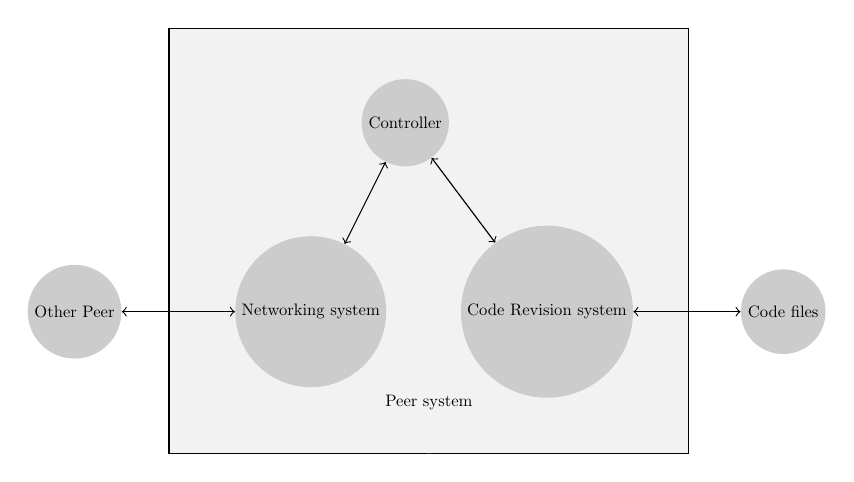
\begin{tikzpicture}[ scale=0.6,transform shape]
\tikzstyle{every node}=[circle,fill=gray!40]
\draw [fill=gray!10] (-3,-3) rectangle (8,6);
\draw (2.5,-3) node [above ,fill=gray!10] {Peer system};
\node (a) at (0,0) {Networking system} ;
\node (b) at (5,0) {Code Revision system};
\node (c) at (2,4) {Controller};
\node (f) at (10,0) {Code files};
\node (u) at (-5,0) {Other Peer};
\draw [<->] (c) -- (a);
\draw [<->] (c) -- (b);
\draw [<->] (u) -- (a);
\draw [<->] (b) -- (f);
\end{tikzpicture}
\caption{Highlevel design}
\end{wrapfigure}

Networking subsystem implements the underlying communication between the
peers using the RPC like framwork. It usually serves therse purposes
\begin{itemize}
\item Defining the underlying protocol for communication.
\item Connecting to a peer and transferring the patches reported by the
  revision system.
\item Interacting with the Code revision system.
\end{itemize}
We have used the python twisted library to implement our networking
system. Twisted's perspective broker (PB) \cite{PB} module provides framework to quickly
and easily implement peer to peer systems. Spread is a kind of RPC (Remote
procedural Calls) which allows us to make remote function calls. The
parameters of the functions as well as the returned element must have
serializable instances. It also allows to pass objects (which inherit from
Copyable class) as parameters to function calls.

The programming style for implementing PB application is asynchronous. It
adds callback to all the remote calls. The call methods are invocated when the
remote procedure returns the result. Thus it ensures that the execution at the
client side continues while the execution of the remote procedure is taking
place. We can also add the error callback which is invocated when an error is
raised at the server side. Thus the remote calls add some bit of transparency
avoiding any overhead due to network latency by being asynchronous.

\pagebreak

\subsection{Code Revision System}

Code Revision system performs all the major tasks of actually interacting with
the code files while keeping track of various versions of the code. It consists of
\begin{itemize}
\item Keeping tracks of all the files added to version control.
\item Creating commit snapshots.
\item At the time of pull/push it determines what commits need to be sent to the remote.
\item Performing merging of code files based on the defined merge strategy.
\end{itemize}
\subsubsection{3 Way  Merge Strategy}
\begin{wrapfigure}[6]{r}{6cm}
\centering
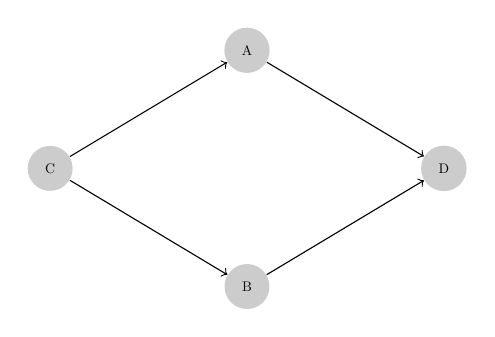
\begin{tikzpicture}[ scale=0.5,transform shape]
\tikzstyle{every node}=[circle,thick,fill=gray!40,inner sep=8]
\node (a) at (0,0) {C} ;
\node (b) at (5,-3) {B};
\node (c) at (5,3) {A};
\node (d) at (10,0) {D};
\draw [->] (a) -- (b);
\draw [->] (a) -- (c);
\draw [->] (b) -- (d);
\draw [->] (c) -- (d);
\end{tikzpicture}
\caption{3-way Merging}
\end{wrapfigure}
There are several reasons which require us to use an automated merge tool for
a distributed revision control system:
\begin{itemize}
\item It is very much possible for two different developers to edit the same
  file in their respective code bases. Then it is very difficult to manually
  merge the two files at the time of combining their versions of code.
\item We want the non-conflicting changes in the same file to get merged
  automatically without any user intervention.
\end{itemize}

There are many merging startegies like 2-Way merge, 3-Way merge, patch
commutation of Darcs, 2-Way merge with history of Codeville
etc. \cite{WIKIMERGE}. We have used 3-Way merge in our project, because it
requires a parent file to merge two files and the revision control systems
mostly gurantees existense of such a file.

Consider, two files \emph{A} and \emph{B} with \emph{C} as their parent file
(the file from which both files have diverged). Our merge algorithm analyses
the difference between files \emph{A} and \emph{B} considering into account
the differences of it from their parent \emph{C} to produce the
automatically-merged file \emph{D}.

\subsection{User Interface/Controller}
This will provide the actual interface which user will be able to use and this
will coordinate the working of the other two components.
It consists of
\begin{itemize}
\item It contains command line interface to perform all the actions. We
  haven't tested it on a windows machine but the code should be portable.
\item An intuitive GUI interface is important to have a better user
  experience, but due to lack of time we could not implement it.
\item We have defined the usual commands like initiate repository, add files,
  pull commits, see log, see the status, revert changes, clone repository,
  push commits etc.
\item This acts like a bridge between the networking subsystem and code
  revision system. It uses both the interfaces to provide an end to end code
  revision system.
\end{itemize}

\subsection{Functionalities}
We are providing the user with the following functionalities:
\begin{itemize}
\item \emph{Init} This command initializes all the directories and files which are required to do the revision control, and asks the user for its username and password which behave as the identity of the user for interacting with other users.
\begin{lstlisting}
$ ./file.py -i
Enter username:
rahulaaj
Enter email
rahulajmera91@gmail.com
\end{lstlisting}
\item \emph{Add} The add command adds a file or a directory to the set of files which on commiting gets added to the repository of files which can be shared over the network.It basically prepares the content prepared for the next commit by adding the modified files.
\begin{lstlisting}
$ ./file.py -a sub
/home/rahulaaj/sub/tests.py => File added to tracking
/home/rahulaaj/sub/merge3.py => File added to tracking
\end{lstlisting}
\item \emph{Commit} This command adds the set of all tracking files added, into a repository which can be accessed using the commit tag along with a necessary commit message by the user to describe the new changes in the commit.
\begin{lstlisting}
./file.py -c 'first commit'
\end{lstlisting}
\item \emph{Diff} The diff commands on given the filename prints out the difference of the file from the last commit, with $+$ signifying the line has been added, $-$ suggesting that the line has been removed and no first charachter means the line has not been changed in the file.
\begin{lstlisting}
$ ./file.py -d sub/tests.py
- import os
  import string
+ import time
+ import merge3
  import file
\end{lstlisting}
\item \emph{Status} It prints out the current status of all the files which are modified and are still not being commited, that is will list out all the files which needs to be commited in order to get stored in the commited file database.
\begin{lstlisting}
$ ./file.py -s
modified: sub/tests.py
\end{lstlisting}
\item \emph{Log} It lists outs the details in the commit log, including the commit tag, author, email and date of all the commits.
\begin{lstlisting}
$ ./file.py -l
Commit: 4fff2246122f98542c57182d97814c05e8f97c853b03d3c8905
Author: rahulaaj
Email: rahulajmera91@gmail.com
Date: 2012-11-01


Commit: 16d92f8e981a69bdca0a3abc1f40359a0331f7bf8ccb9022fc6
Author: rahulaaj
Email: rahulajmera91@gmail.com
Date: 2012-11-01


\end{lstlisting}
\item \emph{Pull} It will get the last commit from a different user over the network and for each file in the commit it will find out the file in the current directory of the user and the parent file (the file from which both files have diverged) and merge them using our 3-way merge algorithm as defined earlier in the Code Revision System section, and after successfully merging it creates a new commit with new merged files in the current directory.
\begin{lstlisting}
$ ./file.py --pull 127.24.1.166:5000/sub
Merged sub/merge3.py

Merged  sub/tests.py
\end{lstlisting}
\item \emph{Push} It is the converse of the pull command discussed above, it pushes the last commit of the current user, which is in turn pulled by other users.It basically updates the remote references(files) using the local copy of the references and sends the required files.
\begin{lstlisting}
$ ./file.py --push 127.24.1.166:5000/sub

\end{lstlisting}
\end{itemize}
\section{Conclusion and Future Work}
\begin{thebibliography}{99}
\bibitem{wiki}
Distributed Revision Control

\url{http://en.wikipedia.org/wiki/Distributed_revision_control}
\bibitem{git}
Git version control system

\url{http://git-scm.com}
\bibitem{mercurial}
Matt Mackall, \emph{Towards a Better SCM: Revlog and Mercurial} .
\bibitem{darcs}
Judah Jacobson,

\emph{A formalization of Darcs patch theory using inverse
  semigroups}.
\bibitem{bazaar}
GNU Bazaar,

\url{http://wiki.bazaar.canonical.com/}
\bibitem{parable}
Git Parable,

\url{http://tom.preston-werner.com/2009/05/19/the-git-parable.html}
\bibitem{PYVCS}
Using Version Control

\url{http://www.fossee.in/sdes-iitb/using_version_control.html}
\bibitem{PB}
Introduction to Perspective Broker

\url{http://twistedmatrix.com/documents/current/core/howto/pb-intro.html}
\bibitem{KISS}
Keep it Simple, Stupid

\url{http://people.apache.org/~fhanik/kiss.html}
\bibitem{WIKIMERGE}
Merge Strategies.

\url{http://en.wikipedia.org/wiki/Merge_%28revision_control%29}
\end{thebibliography}
\end{document}
